
\documentclass[letterpaper,11pt]{article}
\usepackage[utf8]{inputenc}
\usepackage[spanish]{babel}
\usepackage{mathtools}
\usepackage{graphicx}
\usepackage{hyperref}
\usepackage{tikz}

\begin{document}

\title{Estructura de datos\\\Large Montículos binomiales y binarios\\\small Actividad 9}
\author{Dagoberto Quevedo}
\maketitle

\begin{abstract}
En esta actividad se describen las propiedades y funcionalidades de los montículos binomiales y binarios, realizando finalmente un diseño experimental que compara el rendimiento de estas estructuras en una operación de inserción y búsqueda del elemento mínimo.
\end{abstract}

\section{Montículos binarios}

Se define como un árbol binario con las siguientes consideraciones:

\begin{itemize}
\item Todos los niveles del árbol están completos (quizá excepto el último) y si el último nivel del árbol no está completo, los vértice de ese nivel se asignan de izquierda a derecha.

\item La clave almacenada en cada vértice es mayor o igual que ($\geq$) o menor o igual que ($\leq$) las claves en los elementos secundarios del vértice.
\item Los monticulos binarios donde la clave principal es mayor o igual que ($\geq$) las claves secundarias se llaman \textbf{montículo máximo}; aquellos donde es menor o igual a ($\leq$) se llaman \textbf{montículo mínimo}
\end{itemize}

\begin{figure}[h]
 \centering
    \begin{tikzpicture}
     \node [circle,draw]{1} [level distance=10mm,sibling distance=25mm]
    child { node [circle,draw]{2} [level distance=10mm ,sibling distance=15mm]
    child {node [circle,draw] {17}
    child {node [circle,draw] {23}}
    child {node [circle,draw]{86}}}
    child {node [circle,draw]{19}}
    }
    child {node [circle,draw] {3} [level distance=10mm ,sibling distance=15mm]
    child {node [circle,draw] {33}}
    child {node [circle,draw]{9}}
    };
    \end{tikzpicture}
  \caption{Ejemplo de un montículo mínimo binario}
  \label{fig:bs}
\end{figure}

\section{Montículos binómico}

Un montículo binómico se define de una manera recursiva. Un árbol binómico de un vértice es $B_0$ y el único vértice es la raíz. El árbol $B_{k+1}$ contiene dos copias de $B_k$ tal que la raíz de una copia es la raíz de $B:k+1$ y la raíz de la otra copia es un hijo directo de esta raíz Algunas consecuencias de esta definición son que: a) El árbol $B_k$ contiene $2_k$ vértices, b) La altura de $B_k$ es $k$. La raíz de $B_k$ tiene $k$ hijos directos, $B_{k-1}, B_{k-2}, \dots, B_1, B_0$.

Las claves son almacenadas en un árbol binómico según el orden de montículo: la clave del vértice padre es menor que la clave de su hijo. Cada vértice contiene una clave. Un montículo binómico es un conjunto de árboles binómicos tal que no hay duplicados de los $B_k$. \cite{Schaeffer2020} 

\section{Operaciones con montículos}

La siguiente tabla resume el orden de operaciones requeridos para las operación usuales en montículos.

\begin{table}[h!]
\centering
\begin{tabular}{l|c|c}
Operación   & Binario & Binómico \\\hline
Inserción   &  $\mathcal{O}(\log n)$      & $\mathcal{O}(\log n)$       \\
Minímo      & $\mathcal{O}(1)$       & $\mathcal{O}(\log n)$        \\
Unión       & $\mathcal{O}(n)$       & $\mathcal{O}(\log n)$       \\
Eliminación & $\mathcal{O}(\log n)$     & $\mathcal{O}(\log n)$      
\end{tabular}
\label{tbl:ope}
\end{table}


\section{Implementación computacional}

Se realiza la implementación computacional en Python de las estructuras de un montículo binómico y binario. Para el montículo binario se hace uso de la librería \texttt{binary\_heap}, para la implementación del montículo binómico se hace uso del código disponible en \cite{Nayuki2018}. 

\subsection{Condiciones de experimentación}
Se mide el rendimiento en las operaciones de inserción y búsqueda del elemento mínimo en cada estructura. La evaluación se realiza con una serie de instancias, en este caso cada instancia se define como un vector con elementos enteros de tamaño ${2^n}$, donde $n\in \{1,\dots,20\}$, la ejecución se repite $k=10$ veces, con este vector se realiza la inserción iterativa y al finalizar la búsqueda del elemento mínimo.

\subsection{Resultados}
El gráfico \ref{fig:bs} muestra los resultados del diseño experimental en el tiempo de computo expresado en escala logarítmica, el eje vertical expresa el valor de $n$ que define el tamaño de la instancia ${2^n}$. 

\begin{figure}[h]
 \centering
  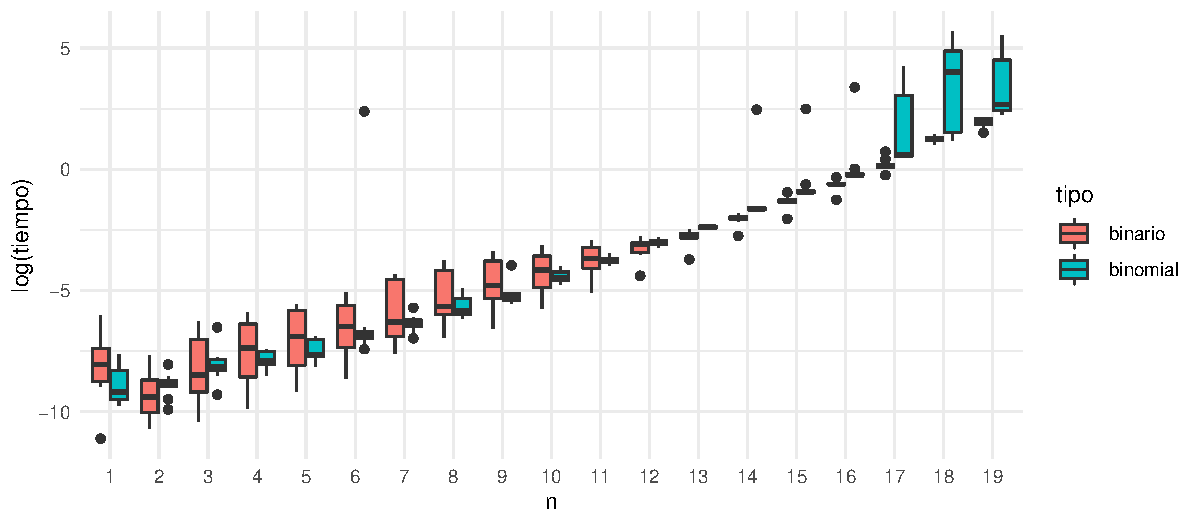
\includegraphics[width=11.5cm]{img/A9_boxplot.pdf}
  \caption{Resultados del diseño experimental con $k=10$ ejecuciones para cada tipo de estructura}
  \label{fig:bs}
\end{figure}

\subsection{Conclusiones}

El montículo binario muestra un rendimiento superior para las operaciones asignadas, siendo consistente con tiempo en orden de operaciones requeridos para cada operación descrito en la tabla \ref{bl:ope}. Cabe señalar que el gráfico no muestra aun que el experimento alcanzo zona asintótica por lo que es requerido ampliar el tamaño del experimento de tal manera de tener resultados concluyentes.




\begin{thebibliography}{0}
  \bibitem{Nayuki2018} \textit{Binomial heap},  Project Nayuki, \url{https://www.nayuki.io/page/binomial-heap} 
  \bibitem{Knuth1998} Donald Knuth, \textit{Sorting and searching}, The Art of Computer Programming, Addison-Wesley Professional, 1998.
  \bibitem{Schaeffer2020} Elisa Schaeffer, \textit{Modelos computacionales}, Complejidad computacional de problemas y el análisis y diseño de algoritmos, notas de curso, 2020.
\end{thebibliography}


\end{document}
